\documentclass[1p]{elsarticle_modified}
%\bibliographystyle{elsarticle-num}

%\usepackage[colorlinks]{hyperref}
%\usepackage{abbrmath_seonhwa} %\Abb, \Ascr, \Acal ,\Abf, \Afrak
\usepackage{amsfonts}
\usepackage{amssymb}
\usepackage{amsmath}
\usepackage{amsthm}
\usepackage{scalefnt}
\usepackage{amsbsy}
\usepackage{kotex}
\usepackage{caption}
\usepackage{subfig}
\usepackage{color}
\usepackage{graphicx}
\usepackage{xcolor} %% white, black, red, green, blue, cyan, magenta, yellow
\usepackage{float}
\usepackage{setspace}
\usepackage{hyperref}

\usepackage{tikz}
\usetikzlibrary{arrows}

\usepackage{multirow}
\usepackage{array} % fixed length table
\usepackage{hhline}

%%%%%%%%%%%%%%%%%%%%%
\makeatletter
\renewcommand*\env@matrix[1][\arraystretch]{%
	\edef\arraystretch{#1}%
	\hskip -\arraycolsep
	\let\@ifnextchar\new@ifnextchar
	\array{*\c@MaxMatrixCols c}}
\makeatother %https://tex.stackexchange.com/questions/14071/how-can-i-increase-the-line-spacing-in-a-matrix
%%%%%%%%%%%%%%%

\usepackage[normalem]{ulem}

\newcommand{\msout}[1]{\ifmmode\text{\sout{\ensuremath{#1}}}\else\sout{#1}\fi}
%SOURCE: \msout is \stkout macro in https://tex.stackexchange.com/questions/20609/strikeout-in-math-mode

\newcommand{\cancel}[1]{
	\ifmmode
	{\color{red}\msout{#1}}
	\else
	{\color{red}\sout{#1}}
	\fi
}

\newcommand{\add}[1]{
	{\color{blue}\uwave{#1}}
}

\newcommand{\replace}[2]{
	\ifmmode
	{\color{red}\msout{#1}}{\color{blue}\uwave{#2}}
	\else
	{\color{red}\sout{#1}}{\color{blue}\uwave{#2}}
	\fi
}

\newcommand{\Sol}{\mathcal{S}} %segment
\newcommand{\D}{D} %diagram
\newcommand{\A}{\mathcal{A}} %arc


%%%%%%%%%%%%%%%%%%%%%%%%%%%%%5 test

\def\sl{\operatorname{\textup{SL}}(2,\Cbb)}
\def\psl{\operatorname{\textup{PSL}}(2,\Cbb)}
\def\quan{\mkern 1mu \triangleright \mkern 1mu}

\theoremstyle{definition}
\newtheorem{thm}{Theorem}[section]
\newtheorem{prop}[thm]{Proposition}
\newtheorem{lem}[thm]{Lemma}
\newtheorem{ques}[thm]{Question}
\newtheorem{cor}[thm]{Corollary}
\newtheorem{defn}[thm]{Definition}
\newtheorem{exam}[thm]{Example}
\newtheorem{rmk}[thm]{Remark}
\newtheorem{alg}[thm]{Algorithm}

\newcommand{\I}{\sqrt{-1}}
\begin{document}

%\begin{frontmatter}
%
%\title{Boundary parabolic representations of knots up to 8 crossings}
%
%%% Group authors per affiliation:
%\author{Yunhi Cho} 
%\address{Department of Mathematics, University of Seoul, Seoul, Korea}
%\ead{yhcho@uos.ac.kr}
%
%
%\author{Seonhwa Kim} %\fnref{s_kim}}
%\address{Center for Geometry and Physics, Institute for Basic Science, Pohang, 37673, Korea}
%\ead{ryeona17@ibs.re.kr}
%
%\author{Hyuk Kim}
%\address{Department of Mathematical Sciences, Seoul National University, Seoul 08826, Korea}
%\ead{hyukkim@snu.ac.kr}
%
%\author{Seokbeom Yoon}
%\address{Department of Mathematical Sciences, Seoul National University, Seoul, 08826,  Korea}
%\ead{sbyoon15@snu.ac.kr}
%
%\begin{abstract}
%We find all boundary parabolic representation of knots up to 8 crossings.
%
%\end{abstract}
%\begin{keyword}
%    \MSC[2010] 57M25 
%\end{keyword}
%
%\end{frontmatter}

%\linenumbers
%\tableofcontents
%
\newcommand\colored[1]{\textcolor{white}{\rule[-0.35ex]{0.8em}{1.4ex}}\kern-0.8em\color{red} #1}%
%\newcommand\colored[1]{\textcolor{white}{ #1}\kern-2.17ex	\textcolor{white}{ #1}\kern-1.81ex	\textcolor{white}{ #1}\kern-2.15ex\color{red}#1	}

{\Large $\underline{11a_{96}~(K11a_{96})}$}

\setlength{\tabcolsep}{10pt}
\renewcommand{\arraystretch}{1.6}
\vspace{1cm}\begin{tabular}{m{100pt}>{\centering\arraybackslash}m{274pt}}
\multirow{5}{120pt}{
	\centering
	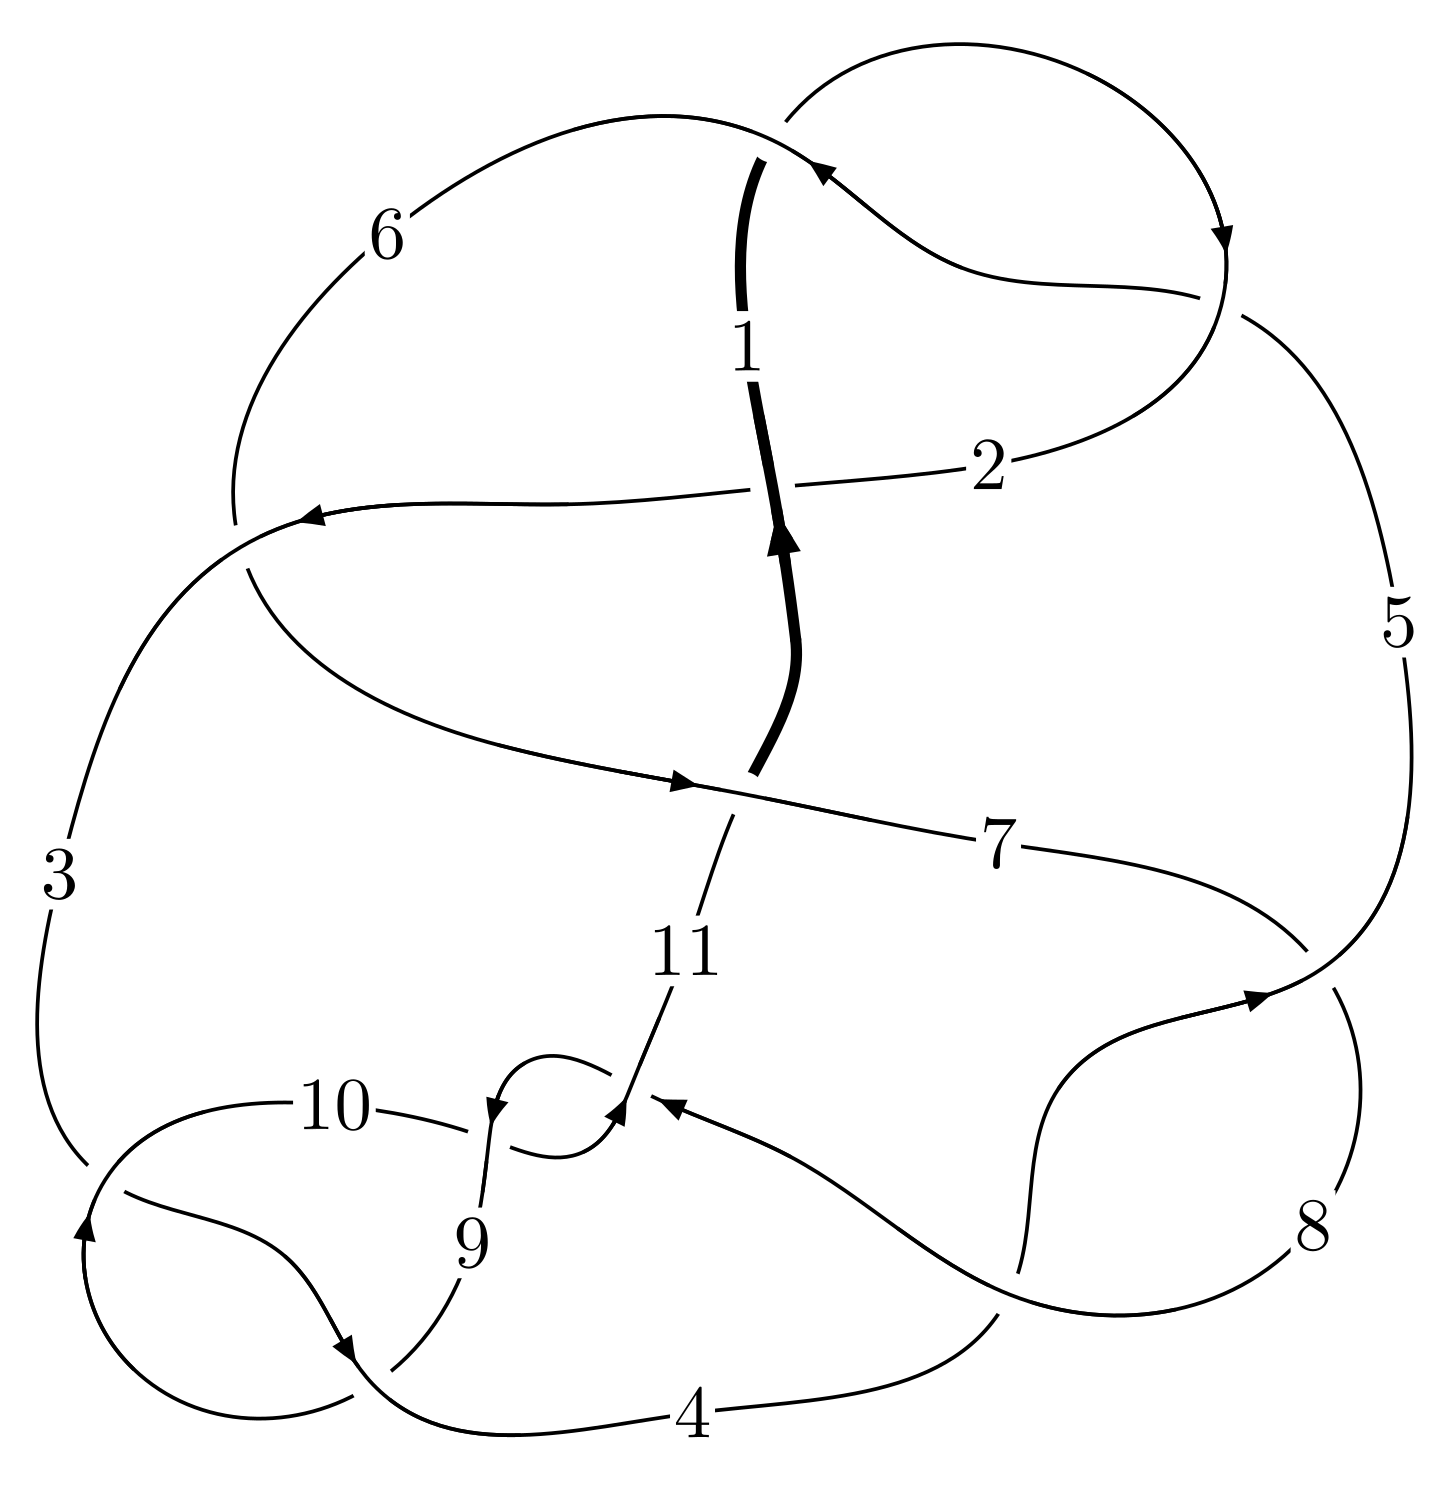
\includegraphics[width=112pt]{../../../GIT/diagram.site/Diagrams/png/345_11a_96.png}\\
\ \ \ A knot diagram\footnotemark}&
\allowdisplaybreaks
\textbf{Linearized knot diagam} \\
\cline{2-2}
 &
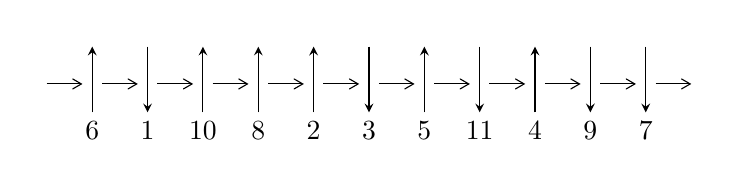
\begin{tikzpicture}[x=20pt, y=17pt]
	% nodes
	\node (C0) at (0, 0) {};
	\node (C1) at (1, 0) {};
	\node (C1U) at (1, +1) {};
	\node (C1D) at (1, -1) {6};

	\node (C2) at (2, 0) {};
	\node (C2U) at (2, +1) {};
	\node (C2D) at (2, -1) {1};

	\node (C3) at (3, 0) {};
	\node (C3U) at (3, +1) {};
	\node (C3D) at (3, -1) {10};

	\node (C4) at (4, 0) {};
	\node (C4U) at (4, +1) {};
	\node (C4D) at (4, -1) {8};

	\node (C5) at (5, 0) {};
	\node (C5U) at (5, +1) {};
	\node (C5D) at (5, -1) {2};

	\node (C6) at (6, 0) {};
	\node (C6U) at (6, +1) {};
	\node (C6D) at (6, -1) {3};

	\node (C7) at (7, 0) {};
	\node (C7U) at (7, +1) {};
	\node (C7D) at (7, -1) {5};

	\node (C8) at (8, 0) {};
	\node (C8U) at (8, +1) {};
	\node (C8D) at (8, -1) {11};

	\node (C9) at (9, 0) {};
	\node (C9U) at (9, +1) {};
	\node (C9D) at (9, -1) {4};

	\node (C10) at (10, 0) {};
	\node (C10U) at (10, +1) {};
	\node (C10D) at (10, -1) {9};

	\node (C11) at (11, 0) {};
	\node (C11U) at (11, +1) {};
	\node (C11D) at (11, -1) {7};
	\node (C12) at (12, 0) {};

	% arrows
	\draw[->,>={angle 60}]
	(C0) edge (C1) (C1) edge (C2) (C2) edge (C3) (C3) edge (C4) (C4) edge (C5) (C5) edge (C6) (C6) edge (C7) (C7) edge (C8) (C8) edge (C9) (C9) edge (C10) (C10) edge (C11) (C11) edge (C12) ;	\draw[->,>=stealth]
	(C1D) edge (C1U) (C2U) edge (C2D) (C3D) edge (C3U) (C4D) edge (C4U) (C5D) edge (C5U) (C6U) edge (C6D) (C7D) edge (C7U) (C8U) edge (C8D) (C9D) edge (C9U) (C10U) edge (C10D) (C11U) edge (C11D) ;
	\end{tikzpicture} \\
\hhline{~~} \\& 
\textbf{Solving Sequence} \\ \cline{2-2} 
 &
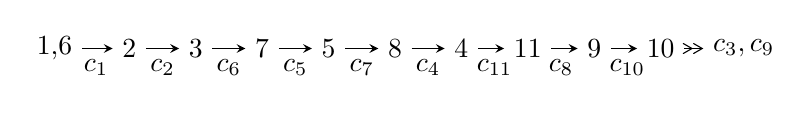
\begin{tikzpicture}[x=24pt, y=7pt]
	% node
	\node (A0) at (-1/8, 0) {1,6};
	\node (A1) at (1, 0) {2};
	\node (A2) at (2, 0) {3};
	\node (A3) at (3, 0) {7};
	\node (A4) at (4, 0) {5};
	\node (A5) at (5, 0) {8};
	\node (A6) at (6, 0) {4};
	\node (A7) at (7, 0) {11};
	\node (A8) at (8, 0) {9};
	\node (A9) at (9, 0) {10};
	\node (C1) at (1/2, -1) {$c_{1}$};
	\node (C2) at (3/2, -1) {$c_{2}$};
	\node (C3) at (5/2, -1) {$c_{6}$};
	\node (C4) at (7/2, -1) {$c_{5}$};
	\node (C5) at (9/2, -1) {$c_{7}$};
	\node (C6) at (11/2, -1) {$c_{4}$};
	\node (C7) at (13/2, -1) {$c_{11}$};
	\node (C8) at (15/2, -1) {$c_{8}$};
	\node (C9) at (17/2, -1) {$c_{10}$};
	\node (A10) at (41/4, 0) {$c_{3},c_{9}$};

	% edge
	\draw[->,>=stealth]	
	(A0) edge (A1) (A1) edge (A2) (A2) edge (A3) (A3) edge (A4) (A4) edge (A5) (A5) edge (A6) (A6) edge (A7) (A7) edge (A8) (A8) edge (A9) ;
	\draw[->>,>={angle 60}]	
	(A9) edge (A10);
\end{tikzpicture} \\ 

\end{tabular} \\

\footnotetext{
The image of knot diagram is generated by the software ``\textbf{Draw programme}" developed by Andrew Bartholomew(\url{http://www.layer8.co.uk/maths/draw/index.htm\#Running-draw}), where we modified some parts for our purpose(\url{https://github.com/CATsTAILs/LinksPainter}).
}\phantom \\ \newline 
\centering \textbf{Ideals for irreducible components\footnotemark of $X_{\text{par}}$} 
 
\begin{align*}
I^u_{1}&=\langle 
u^{60}- u^{59}+\cdots+u^2+1\rangle \\
\\
\end{align*}
\raggedright * 1 irreducible components of $\dim_{\mathbb{C}}=0$, with total 60 representations.\\
\footnotetext{All coefficients of polynomials are rational numbers. But the coefficients are sometimes approximated in decimal forms when there is not enough margin.}
\newpage
\renewcommand{\arraystretch}{1}
\centering \section*{I. $I^u_{1}= \langle u^{60}- u^{59}+\cdots+u^2+1 \rangle$}
\flushleft \textbf{(i) Arc colorings}\\
\begin{tabular}{m{7pt} m{180pt} m{7pt} m{180pt} }
\flushright $a_{1}=$&$\begin{pmatrix}1\\0\end{pmatrix}$ \\
\flushright $a_{6}=$&$\begin{pmatrix}0\\u\end{pmatrix}$ \\
\flushright $a_{2}=$&$\begin{pmatrix}1\\- u^2\end{pmatrix}$ \\
\flushright $a_{3}=$&$\begin{pmatrix}u^2+1\\- u^2\end{pmatrix}$ \\
\flushright $a_{7}=$&$\begin{pmatrix}- u^5-2 u^3- u\\u^5+u^3+u\end{pmatrix}$ \\
\flushright $a_{5}=$&$\begin{pmatrix}- u\\u^3+u\end{pmatrix}$ \\
\flushright $a_{8}=$&$\begin{pmatrix}- u^9-2 u^7-3 u^5-2 u^3- u\\u^{11}+3 u^9+4 u^7+3 u^5+u^3+u\end{pmatrix}$ \\
\flushright $a_{4}=$&$\begin{pmatrix}- u^{17}-4 u^{15}-9 u^{13}-12 u^{11}-11 u^9-6 u^7-2 u^5- u\\u^{19}+5 u^{17}+12 u^{15}+17 u^{13}+15 u^{11}+9 u^9+4 u^7+2 u^5+u^3+u\end{pmatrix}$ \\
\flushright $a_{11}=$&$\begin{pmatrix}u^{10}+3 u^8+4 u^6+3 u^4+u^2+1\\- u^{10}-2 u^8-3 u^6-2 u^4- u^2\end{pmatrix}$ \\
\flushright $a_{9}=$&$\begin{pmatrix}- u^{31}-8 u^{29}+\cdots-4 u^3-2 u\\u^{31}+7 u^{29}+\cdots+2 u^3+u\end{pmatrix}$ \\
\flushright $a_{10}=$&$\begin{pmatrix}u^{52}+13 u^{50}+\cdots+3 u^2+1\\- u^{52}-12 u^{50}+\cdots-5 u^4-2 u^2\end{pmatrix}$\\ \flushright $a_{10}=$&$\begin{pmatrix}u^{52}+13 u^{50}+\cdots+3 u^2+1\\- u^{52}-12 u^{50}+\cdots-5 u^4-2 u^2\end{pmatrix}$\\&\end{tabular}
\flushleft \textbf{(ii) Obstruction class $= -1$}\\~\\
\flushleft \textbf{(iii) Cusp Shapes $= -4 u^{59}+4 u^{58}+\cdots-4 u+2$}\\~\\
\newpage\renewcommand{\arraystretch}{1}
\flushleft \textbf{(iv) u-Polynomials at the component}\newline \\
\begin{tabular}{m{50pt}|m{274pt}}
Crossings & \hspace{64pt}u-Polynomials at each crossing \\
\hline $$\begin{aligned}c_{1},c_{5}\end{aligned}$$&$\begin{aligned}
&u^{60}- u^{59}+\cdots+u^2+1
\end{aligned}$\\
\hline $$\begin{aligned}c_{2}\end{aligned}$$&$\begin{aligned}
&u^{60}+29 u^{59}+\cdots+2 u+1
\end{aligned}$\\
\hline $$\begin{aligned}c_{3},c_{9}\end{aligned}$$&$\begin{aligned}
&u^{60}- u^{59}+\cdots+u^2+1
\end{aligned}$\\
\hline $$\begin{aligned}c_{4},c_{7}\end{aligned}$$&$\begin{aligned}
&u^{60}+5 u^{59}+\cdots+122 u+13
\end{aligned}$\\
\hline $$\begin{aligned}c_{6}\end{aligned}$$&$\begin{aligned}
&u^{60}+u^{59}+\cdots-118 u+37
\end{aligned}$\\
\hline $$\begin{aligned}c_{8},c_{10}\end{aligned}$$&$\begin{aligned}
&u^{60}+21 u^{59}+\cdots+2 u+1
\end{aligned}$\\
\hline $$\begin{aligned}c_{11}\end{aligned}$$&$\begin{aligned}
&u^{60}-5 u^{59}+\cdots-12 u+1
\end{aligned}$\\
\hline
\end{tabular}\\~\\
\newpage\renewcommand{\arraystretch}{1}
\flushleft \textbf{(v) Riley Polynomials at the component}\newline \\
\begin{tabular}{m{50pt}|m{274pt}}
Crossings & \hspace{64pt}Riley Polynomials at each crossing \\
\hline $$\begin{aligned}c_{1},c_{5}\end{aligned}$$&$\begin{aligned}
&y^{60}+29 y^{59}+\cdots+2 y+1
\end{aligned}$\\
\hline $$\begin{aligned}c_{2}\end{aligned}$$&$\begin{aligned}
&y^{60}+5 y^{59}+\cdots+14 y+1
\end{aligned}$\\
\hline $$\begin{aligned}c_{3},c_{9}\end{aligned}$$&$\begin{aligned}
&y^{60}+21 y^{59}+\cdots+2 y+1
\end{aligned}$\\
\hline $$\begin{aligned}c_{4},c_{7}\end{aligned}$$&$\begin{aligned}
&y^{60}+41 y^{59}+\cdots+4330 y+169
\end{aligned}$\\
\hline $$\begin{aligned}c_{6}\end{aligned}$$&$\begin{aligned}
&y^{60}-19 y^{59}+\cdots+12050 y+1369
\end{aligned}$\\
\hline $$\begin{aligned}c_{8},c_{10}\end{aligned}$$&$\begin{aligned}
&y^{60}+37 y^{59}+\cdots+22 y+1
\end{aligned}$\\
\hline $$\begin{aligned}c_{11}\end{aligned}$$&$\begin{aligned}
&y^{60}+y^{59}+\cdots+38 y+1
\end{aligned}$\\
\hline
\end{tabular}\\~\\
\newpage\flushleft \textbf{(vi) Complex Volumes and Cusp Shapes}
$$\begin{array}{c|c|c}  
\text{Solutions to }I^u_{1}& \I (\text{vol} + \sqrt{-1}CS) & \text{Cusp shape}\\
 \hline 
\begin{aligned}
u &= -0.544109 + 0.871535 I\end{aligned}
 & \phantom{-}0.80579 + 3.33102 I & \phantom{-}2.01338 - 1.91534 I \\ \hline\begin{aligned}
u &= -0.544109 - 0.871535 I\end{aligned}
 & \phantom{-}0.80579 - 3.33102 I & \phantom{-}2.01338 + 1.91534 I \\ \hline\begin{aligned}
u &= \phantom{-}0.525209 + 0.910684 I\end{aligned}
 & \phantom{-}1.69680 + 2.03222 I & \phantom{-}3.90722 - 3.29370 I \\ \hline\begin{aligned}
u &= \phantom{-}0.525209 - 0.910684 I\end{aligned}
 & \phantom{-}1.69680 - 2.03222 I & \phantom{-}3.90722 + 3.29370 I \\ \hline\begin{aligned}
u &= -0.622652 + 0.677380 I\end{aligned}
 & \phantom{-}1.38479 - 7.95567 I & \phantom{-}3.11940 + 8.08739 I \\ \hline\begin{aligned}
u &= -0.622652 - 0.677380 I\end{aligned}
 & \phantom{-}1.38479 + 7.95567 I & \phantom{-}3.11940 - 8.08739 I \\ \hline\begin{aligned}
u &= -0.552672 + 0.728082 I\end{aligned}
 & -3.08637 - 2.17441 I & -2.78142 + 3.98454 I \\ \hline\begin{aligned}
u &= -0.552672 - 0.728082 I\end{aligned}
 & -3.08637 + 2.17441 I & -2.78142 - 3.98454 I \\ \hline\begin{aligned}
u &= -0.074861 + 0.899343 I\end{aligned}
 & \phantom{-}0.55103 + 2.51832 I & -0.80649 - 3.33072 I \\ \hline\begin{aligned}
u &= -0.074861 - 0.899343 I\end{aligned}
 & \phantom{-}0.55103 - 2.51832 I & -0.80649 + 3.33072 I \\ \hline\begin{aligned}
u &= \phantom{-}0.610444 + 0.652587 I\end{aligned}
 & \phantom{-}2.44765 + 2.49685 I & \phantom{-}5.32046 - 3.18664 I \\ \hline\begin{aligned}
u &= \phantom{-}0.610444 - 0.652587 I\end{aligned}
 & \phantom{-}2.44765 - 2.49685 I & \phantom{-}5.32046 + 3.18664 I \\ \hline\begin{aligned}
u &= -0.381105 + 1.041640 I\end{aligned}
 & -3.34743 - 1.08708 I & -6.46120 + 0. I\phantom{ +0.000000I} \\ \hline\begin{aligned}
u &= -0.381105 - 1.041640 I\end{aligned}
 & -3.34743 + 1.08708 I & -6.46120 + 0. I\phantom{ +0.000000I} \\ \hline\begin{aligned}
u &= \phantom{-}0.484539 + 1.021160 I\end{aligned}
 & -0.56534 + 3.02304 I & \phantom{-0.000000 } 0 \\ \hline\begin{aligned}
u &= \phantom{-}0.484539 - 1.021160 I\end{aligned}
 & -0.56534 - 3.02304 I & \phantom{-0.000000 } 0 \\ \hline\begin{aligned}
u &= -0.260652 + 1.137700 I\end{aligned}
 & -3.60470 + 1.42729 I & \phantom{-0.000000 } 0 \\ \hline\begin{aligned}
u &= -0.260652 - 1.137700 I\end{aligned}
 & -3.60470 - 1.42729 I & \phantom{-0.000000 } 0 \\ \hline\begin{aligned}
u &= -0.313837 + 1.128650 I\end{aligned}
 & -4.20665 - 1.05171 I & \phantom{-0.000000 } 0 \\ \hline\begin{aligned}
u &= -0.313837 - 1.128650 I\end{aligned}
 & -4.20665 + 1.05171 I & \phantom{-0.000000 } 0 \\ \hline\begin{aligned}
u &= \phantom{-}0.769876 + 0.302697 I\end{aligned}
 & -0.43983 - 9.87486 I & \phantom{-}1.61763 + 6.92341 I \\ \hline\begin{aligned}
u &= \phantom{-}0.769876 - 0.302697 I\end{aligned}
 & -0.43983 + 9.87486 I & \phantom{-}1.61763 - 6.92341 I \\ \hline\begin{aligned}
u &= \phantom{-}0.257348 + 1.151700 I\end{aligned}
 & -4.93303 - 6.89109 I & \phantom{-0.000000 } 0 \\ \hline\begin{aligned}
u &= \phantom{-}0.257348 - 1.151700 I\end{aligned}
 & -4.93303 + 6.89109 I & \phantom{-0.000000 } 0 \\ \hline\begin{aligned}
u &= \phantom{-}0.666201 + 0.472083 I\end{aligned}
 & \phantom{-}5.00152 + 1.75323 I & \phantom{-}7.65668 - 2.62236 I \\ \hline\begin{aligned}
u &= \phantom{-}0.666201 - 0.472083 I\end{aligned}
 & \phantom{-}5.00152 - 1.75323 I & \phantom{-}7.65668 + 2.62236 I \\ \hline\begin{aligned}
u &= -0.755668 + 0.307937 I\end{aligned}
 & \phantom{-}0.80884 + 4.33115 I & \phantom{-}3.69848 - 2.33072 I \\ \hline\begin{aligned}
u &= -0.755668 - 0.307937 I\end{aligned}
 & \phantom{-}0.80884 - 4.33115 I & \phantom{-}3.69848 + 2.33072 I \\ \hline\begin{aligned}
u &= \phantom{-}0.560154 + 1.046520 I\end{aligned}
 & \phantom{-}3.31782 + 3.01457 I & \phantom{-0.000000 } 0 \\ \hline\begin{aligned}
u &= \phantom{-}0.560154 - 1.046520 I\end{aligned}
 & \phantom{-}3.31782 - 3.01457 I & \phantom{-0.000000 } 0\\
 \hline 
 \end{array}$$\newpage$$\begin{array}{c|c|c}  
\text{Solutions to }I^u_{1}& \I (\text{vol} + \sqrt{-1}CS) & \text{Cusp shape}\\
 \hline 
\begin{aligned}
u &= -0.679575 + 0.445417 I\end{aligned}
 & \phantom{-}4.87624 + 3.78274 I & \phantom{-}7.16156 - 3.71379 I \\ \hline\begin{aligned}
u &= -0.679575 - 0.445417 I\end{aligned}
 & \phantom{-}4.87624 - 3.78274 I & \phantom{-}7.16156 + 3.71379 I \\ \hline\begin{aligned}
u &= \phantom{-}0.288034 + 1.152760 I\end{aligned}
 & -9.39383 - 0.41865 I & \phantom{-0.000000 } 0 \\ \hline\begin{aligned}
u &= \phantom{-}0.288034 - 1.152760 I\end{aligned}
 & -9.39383 + 0.41865 I & \phantom{-0.000000 } 0 \\ \hline\begin{aligned}
u &= -0.487828 + 1.088330 I\end{aligned}
 & -2.57613 - 5.90818 I & \phantom{-0.000000 } 0 \\ \hline\begin{aligned}
u &= -0.487828 - 1.088330 I\end{aligned}
 & -2.57613 + 5.90818 I & \phantom{-0.000000 } 0 \\ \hline\begin{aligned}
u &= \phantom{-}0.321894 + 1.149490 I\end{aligned}
 & -5.68245 + 6.13484 I & \phantom{-0.000000 } 0 \\ \hline\begin{aligned}
u &= \phantom{-}0.321894 - 1.149490 I\end{aligned}
 & -5.68245 - 6.13484 I & \phantom{-0.000000 } 0 \\ \hline\begin{aligned}
u &= -0.562904 + 1.061080 I\end{aligned}
 & \phantom{-}3.07462 - 8.59241 I & \phantom{-0.000000 } 0 \\ \hline\begin{aligned}
u &= -0.562904 - 1.061080 I\end{aligned}
 & \phantom{-}3.07462 + 8.59241 I & \phantom{-0.000000 } 0 \\ \hline\begin{aligned}
u &= \phantom{-}0.751525 + 0.268257 I\end{aligned}
 & -5.11292 - 3.55390 I & -3.52030 + 2.87156 I \\ \hline\begin{aligned}
u &= \phantom{-}0.751525 - 0.268257 I\end{aligned}
 & -5.11292 + 3.55390 I & -3.52030 - 2.87156 I \\ \hline\begin{aligned}
u &= -0.533131 + 1.124390 I\end{aligned}
 & -2.71521 - 6.69056 I & \phantom{-0.000000 } 0 \\ \hline\begin{aligned}
u &= -0.533131 - 1.124390 I\end{aligned}
 & -2.71521 + 6.69056 I & \phantom{-0.000000 } 0 \\ \hline\begin{aligned}
u &= \phantom{-}0.719744 + 0.218682 I\end{aligned}
 & -1.68268 + 2.83631 I & -0.28832 - 2.76871 I \\ \hline\begin{aligned}
u &= \phantom{-}0.719744 - 0.218682 I\end{aligned}
 & -1.68268 - 2.83631 I & -0.28832 + 2.76871 I \\ \hline\begin{aligned}
u &= \phantom{-}0.523358 + 1.138230 I\end{aligned}
 & -4.31649 + 1.84933 I & \phantom{-0.000000 } 0 \\ \hline\begin{aligned}
u &= \phantom{-}0.523358 - 1.138230 I\end{aligned}
 & -4.31649 - 1.84933 I & \phantom{-0.000000 } 0 \\ \hline\begin{aligned}
u &= \phantom{-}0.493299 + 0.552242 I\end{aligned}
 & \phantom{-}0.862519 + 1.026220 I & \phantom{-}5.84285 - 4.48468 I \\ \hline\begin{aligned}
u &= \phantom{-}0.493299 - 0.552242 I\end{aligned}
 & \phantom{-}0.862519 - 1.026220 I & \phantom{-}5.84285 + 4.48468 I \\ \hline\begin{aligned}
u &= -0.689013 + 0.265335 I\end{aligned}
 & -0.26353 + 1.99974 I & \phantom{-}2.67797 - 3.08609 I \\ \hline\begin{aligned}
u &= -0.689013 - 0.265335 I\end{aligned}
 & -0.26353 - 1.99974 I & \phantom{-}2.67797 + 3.08609 I \\ \hline\begin{aligned}
u &= -0.558377 + 1.131910 I\end{aligned}
 & -1.60310 - 9.28831 I & \phantom{-0.000000 } 0 \\ \hline\begin{aligned}
u &= -0.558377 - 1.131910 I\end{aligned}
 & -1.60310 + 9.28831 I & \phantom{-0.000000 } 0 \\ \hline\begin{aligned}
u &= \phantom{-}0.545235 + 1.140190 I\end{aligned}
 & -7.65214 + 8.43403 I & \phantom{-0.000000 } 0 \\ \hline\begin{aligned}
u &= \phantom{-}0.545235 - 1.140190 I\end{aligned}
 & -7.65214 - 8.43403 I & \phantom{-0.000000 } 0 \\ \hline\begin{aligned}
u &= \phantom{-}0.560770 + 1.137600 I\end{aligned}
 & -2.8910 + 14.8744 I & \phantom{-0.000000 } 0 \\ \hline\begin{aligned}
u &= \phantom{-}0.560770 - 1.137600 I\end{aligned}
 & -2.8910 - 14.8744 I & \phantom{-0.000000 } 0 \\ \hline\begin{aligned}
u &= -0.561245 + 0.222030 I\end{aligned}
 & -0.23326 + 1.74631 I & \phantom{-}0.21628 - 4.30130 I \\ \hline\begin{aligned}
u &= -0.561245 - 0.222030 I\end{aligned}
 & -0.23326 - 1.74631 I & \phantom{-}0.21628 + 4.30130 I\\
 \hline 
 \end{array}$$\newpage
\newpage\renewcommand{\arraystretch}{1}
\centering \section*{ II. u-Polynomials}
\begin{tabular}{m{50pt}|m{274pt}}
Crossings & \hspace{64pt}u-Polynomials at each crossing \\
\hline $$\begin{aligned}c_{1},c_{5}\end{aligned}$$&$\begin{aligned}
&u^{60}- u^{59}+\cdots+u^2+1
\end{aligned}$\\
\hline $$\begin{aligned}c_{2}\end{aligned}$$&$\begin{aligned}
&u^{60}+29 u^{59}+\cdots+2 u+1
\end{aligned}$\\
\hline $$\begin{aligned}c_{3},c_{9}\end{aligned}$$&$\begin{aligned}
&u^{60}- u^{59}+\cdots+u^2+1
\end{aligned}$\\
\hline $$\begin{aligned}c_{4},c_{7}\end{aligned}$$&$\begin{aligned}
&u^{60}+5 u^{59}+\cdots+122 u+13
\end{aligned}$\\
\hline $$\begin{aligned}c_{6}\end{aligned}$$&$\begin{aligned}
&u^{60}+u^{59}+\cdots-118 u+37
\end{aligned}$\\
\hline $$\begin{aligned}c_{8},c_{10}\end{aligned}$$&$\begin{aligned}
&u^{60}+21 u^{59}+\cdots+2 u+1
\end{aligned}$\\
\hline $$\begin{aligned}c_{11}\end{aligned}$$&$\begin{aligned}
&u^{60}-5 u^{59}+\cdots-12 u+1
\end{aligned}$\\
\hline
\end{tabular}\newpage\renewcommand{\arraystretch}{1}
\centering \section*{ III. Riley Polynomials}
\begin{tabular}{m{50pt}|m{274pt}}
Crossings & \hspace{64pt}Riley Polynomials at each crossing \\
\hline $$\begin{aligned}c_{1},c_{5}\end{aligned}$$&$\begin{aligned}
&y^{60}+29 y^{59}+\cdots+2 y+1
\end{aligned}$\\
\hline $$\begin{aligned}c_{2}\end{aligned}$$&$\begin{aligned}
&y^{60}+5 y^{59}+\cdots+14 y+1
\end{aligned}$\\
\hline $$\begin{aligned}c_{3},c_{9}\end{aligned}$$&$\begin{aligned}
&y^{60}+21 y^{59}+\cdots+2 y+1
\end{aligned}$\\
\hline $$\begin{aligned}c_{4},c_{7}\end{aligned}$$&$\begin{aligned}
&y^{60}+41 y^{59}+\cdots+4330 y+169
\end{aligned}$\\
\hline $$\begin{aligned}c_{6}\end{aligned}$$&$\begin{aligned}
&y^{60}-19 y^{59}+\cdots+12050 y+1369
\end{aligned}$\\
\hline $$\begin{aligned}c_{8},c_{10}\end{aligned}$$&$\begin{aligned}
&y^{60}+37 y^{59}+\cdots+22 y+1
\end{aligned}$\\
\hline $$\begin{aligned}c_{11}\end{aligned}$$&$\begin{aligned}
&y^{60}+y^{59}+\cdots+38 y+1
\end{aligned}$\\
\hline
\end{tabular}
\vskip 2pc
\end{document}